% !TEX encoding = UTF-8 Unicode
\section{Einleitung}
\subsection{Motivation}
\begin{figure}[htbp]
	\centering
 	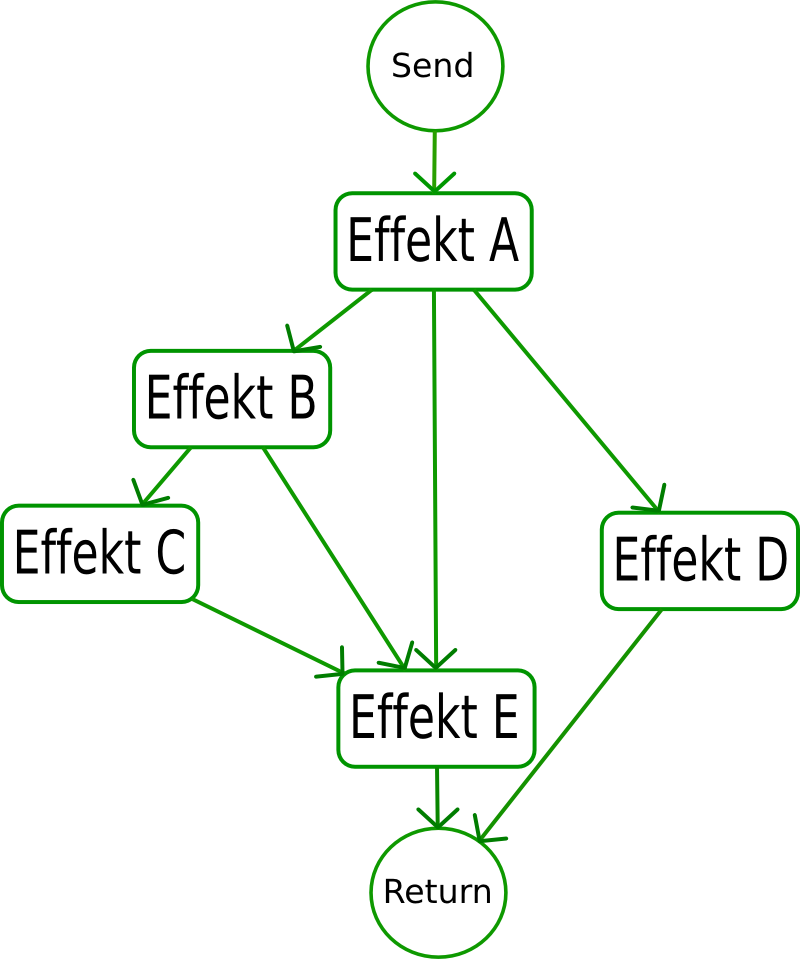
\includegraphics[scale=0.12]{../graphics/free_order}
	\caption{Beispiel einer Effektverkettung, wie sie in der Realität möglich wäre}
	\label{freeOrder}
\end{figure}
Moderne DAWs\footnote{Digital Audio Workstation: computergestütztes System für Tonaufnahme, Musikproduktion, Abmischung und Mastering} bieten umfangreiche und kreative Werkzeuge zum Erzeugen und Manipulieren von Klangereignissen. In vielen Fällen orientierten sich solche Programme anhand real existierender Hardware. So wird oftmals ein Klangereignis einem Kanal in einem virtuellen Mischpult zugeordnet, der einem real existierenden Gerät nachempfunden wurde.
\\\\
Es können neben der Lautstärkeregelung und Stereoverteilung auch Effekte in einen solchen Kanal eingeschliffen werden. Hier unterscheiden sich allerdings die Möglichkeiten zwischen real existierender Hardware und der Software Lösung. Während es in der Realität unzählige Möglichkeiten gibt verschiedene Effekte zu kombinieren - sprich zu „verdrahten“ (siehe Abbildung \ref{freeOrder}) - sind die meisten DAWs in ihren Möglichkeiten beschränkt.
Dies soll anhand des Sequenzers ''Cubase\footnote{verwendete Version: Cubase SL 2.0 ( http://www.steinberg.net )}'' veranschaulicht werden:
\\\\
\begin{figure}[htbp]
	\centering
	\begin{minipage}[b]{7.2 cm}
		
\includegraphics[scale=0.15]{../graphics/send-pre}
	\end{minipage}
	\begin{minipage}[b]{7.2 cm}
 		
\includegraphics[scale=0.15]{../graphics/send-post}
	\end{minipage}
	\caption{Effektkette mit 'send' Abzweigung, jeweils als 'pre' und als 'post' Variante (v.l.n.r)}
	\label{send}
\end{figure}
Jede Klangquelle in Cubase, sei es eine Audiospur oder ein virtuelles Instrument, wird einem eigenen Kanal in dem virtuellen Mischpult zugeordnet. 
Jeder Kanal hat neben einem Equalizer und einer Pan-/Lautstärkeregelung eine feste Anzahl von  ''Insert-Slots''. In einen solchen ''Slot'' kann genau ein Effektmodul geladen werden (in Abbildung 2 und 3 als ''Effekt A..X'' bezeichnet). Jeder dieser Effekte wird nacheinander durchlaufen, was einer Reihenschaltung entspricht. Für eine Parallelschaltung steht eine begrenzte Anzahl von sogenannten ''Send'' Signalwegen zur Verfügung, von denen es zwei Varianten gibt: ''pre-send'' und ''post-send'' (siehe Abbildung \ref{send}).
Je nach Typ wird das Audiosignal vor der Insert-Effektkette abgegriffen oder danach und in einen Effekt Kanal geleitet. Dieser Effektkanal besteht wiederum aus einer begrenzten Anzahl aus ''Insert-Slots''.
\\\\
Diese Möglichkeiten sind für die meisten Produktionen vollkommen ausreichend, da der Unterschied - ob ein Effekt in Reihe oder parallel geschaltet wurde - abhängig vom Effekttyp - meistens sehr gering ist. Dennoch ist es manchmal wünschenswert etwas mehr Kontrolle und Übersicht über die Zusammensetzung der einzelnen Signalwege zu haben. 
\\\\
\begin{figure}[htbp]
	\centering
	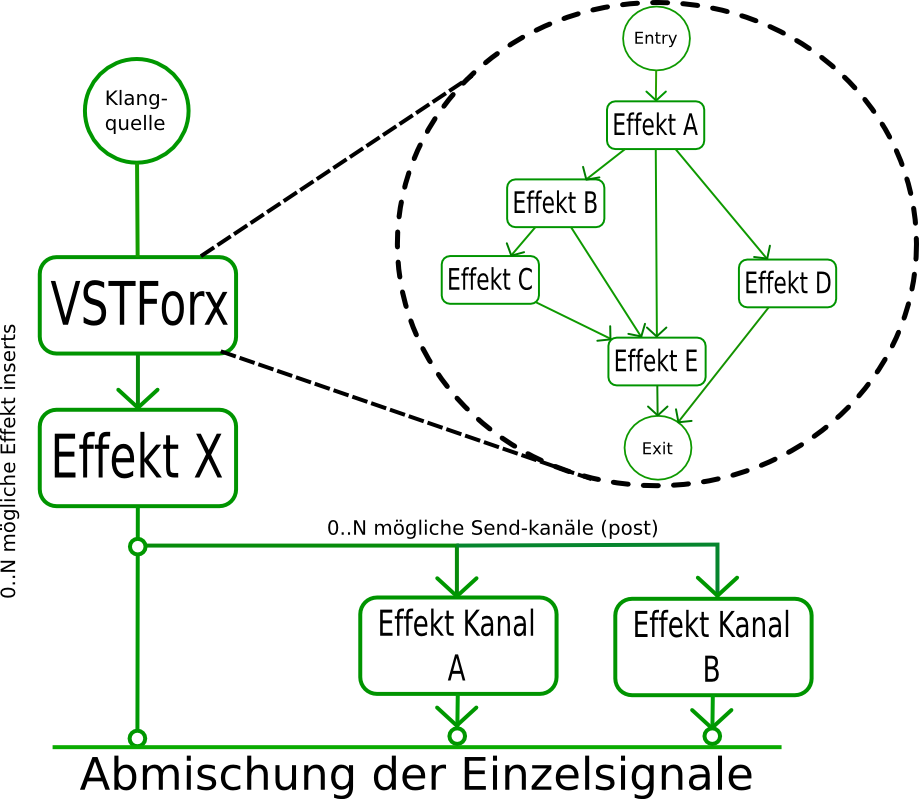
\includegraphics[scale=0.2]{../graphics/solution_vstforx}
 	\caption{Die Idee - freie Verdrahtung als Effekt}
	\label{solutionVSTForx}
\end{figure}
Ziel ist es ein Programm zu entwickeln, das genau das bietet. Es sollte es möglich machen beliebig viele Effekte auf eine virtuelle ''Bühne'' zu laden um diese wiederum beliebig ''verdrahten'' zu können. Das Programm sollte selbst ein Effekt sein. Somit wäre die Integration in eine DAW Umgebung denkbar einfach (siehe Abbildung \ref{solutionVSTForx}).\\
Die meisten Effekte werden durch Parameter gesteuert. Diese Parameter sollten sich ebenfalls in Form von Reglern auf die ''Bühne'' holen und von dort aus bedienen lassen. 
Diese Regler könnte man verbinden und somit mehrere Regler mit einmal steuern. So wäre es zum Beispiel möglich die Intensität eines Halleffektes und die Intensität eines Verzerrers mit einem einzigen Regler gleichzeitig zu steuern.
Darüber hinaus bietet es sich an den Signalfluss und das verhalten der Effekte durch zusätzliche Module manipulierbar beziehungsweise erweiterbar zu machen. Es wäre zum Beispiel eine Art ''Step-Sequencer'' denkbar. Ein Modul welches Rhythmisch zwischen verschiedenen Signalwegen umschaltet. 
\\\\
Das Programm wäre ein ideales Werkzeug zum erschaffen von kreativen Klangexperimenten.
\subsection{Der Name}
Als Programmname entschied ich mich für ''VSTForx''. 
\paragraph{VST} VST\footnote{Abkürzung für ''Virtual Studio Technology'' - Steinberg Media Technologies GmbH} ist eine Plugin-Schnittstelle im Bereich Audioverarbeitung. Aufgrund der hohen Verbreitung von VST-Plugins, wird die zu entwickelnde Software diese Schnittstelle Hauptsächlich unterstützen.
\paragraph{Forx} ein Kunstwort das vom englischen Wort ''fork'' abgeleitet ist. Fork bedeutet Gabelung oder Abzweigung und beschreibt somit ziemlich treffend den Hauptzweck der Software.